\documentclass{article}\usepackage[]{graphicx}\usepackage[]{color}
% maxwidth is the original width if it is less than linewidth
% otherwise use linewidth (to make sure the graphics do not exceed the margin)
\makeatletter
\def\maxwidth{ %
  \ifdim\Gin@nat@width>\linewidth
    \linewidth
  \else
    \Gin@nat@width
  \fi
}
\makeatother

\definecolor{fgcolor}{rgb}{0.196, 0.196, 0.196}
\newcommand{\hlnum}[1]{\textcolor[rgb]{0.063,0.58,0.627}{#1}}%
\newcommand{\hlstr}[1]{\textcolor[rgb]{0.063,0.58,0.627}{#1}}%
\newcommand{\hlcom}[1]{\textcolor[rgb]{0.588,0.588,0.588}{#1}}%
\newcommand{\hlopt}[1]{\textcolor[rgb]{0.196,0.196,0.196}{#1}}%
\newcommand{\hlstd}[1]{\textcolor[rgb]{0.196,0.196,0.196}{#1}}%
\newcommand{\hlkwa}[1]{\textcolor[rgb]{0.231,0.416,0.784}{#1}}%
\newcommand{\hlkwb}[1]{\textcolor[rgb]{0.627,0,0.314}{#1}}%
\newcommand{\hlkwc}[1]{\textcolor[rgb]{0,0.631,0.314}{#1}}%
\newcommand{\hlkwd}[1]{\textcolor[rgb]{0.78,0.227,0.412}{#1}}%
\let\hlipl\hlkwb

\usepackage{framed}
\makeatletter
\newenvironment{kframe}{%
 \def\at@end@of@kframe{}%
 \ifinner\ifhmode%
  \def\at@end@of@kframe{\end{minipage}}%
  \begin{minipage}{\columnwidth}%
 \fi\fi%
 \def\FrameCommand##1{\hskip\@totalleftmargin \hskip-\fboxsep
 \colorbox{shadecolor}{##1}\hskip-\fboxsep
     % There is no \\@totalrightmargin, so:
     \hskip-\linewidth \hskip-\@totalleftmargin \hskip\columnwidth}%
 \MakeFramed {\advance\hsize-\width
   \@totalleftmargin\z@ \linewidth\hsize
   \@setminipage}}%
 {\par\unskip\endMakeFramed%
 \at@end@of@kframe}
\makeatother

\definecolor{shadecolor}{rgb}{.97, .97, .97}
\definecolor{messagecolor}{rgb}{0, 0, 0}
\definecolor{warningcolor}{rgb}{1, 0, 1}
\definecolor{errorcolor}{rgb}{1, 0, 0}
\newenvironment{knitrout}{}{} % an empty environment to be redefined in TeX

\usepackage{alltt}
\usepackage{geometry}
\geometry{a4paper, margin=0.75in}
\usepackage{amsmath,amsthm,amssymb}
\usepackage{bm}
\usepackage{graphicx}
\usepackage[dvipsnames]{xcolor}
\usepackage{multicol}
\usepackage{multirow}
\usepackage{float}
\usepackage{siunitx}
\usepackage{xr}
\externaldocument[sup:]{supplement}
\usepackage[hidelinks]{hyperref}
\usepackage{cleveref}
\usepackage{authblk}
\usepackage{booktabs}
\usepackage{array}
\usepackage{colortbl}
\usepackage[]{caption}
\sisetup{output-exponent-marker=\ensuremath{\mathrm{e}}}

%% Supplemental figure notation
\renewcommand\thefigure{S\arabic{figure}}
\renewcommand\thetable{S\arabic{table}}

%% shortcuts
\newcommand{\pr}[2][]{\text{Pr}_{#1}\left\{#2\right\}}
\newcommand{\E}[2][]{\text{E}_{#1}\left[#2\right]}
\newcommand{\Var}[2][]{\text{Var}_{#1}\left(#2\right)}
\newcommand\I[1]{\text{I}\left(#1\right)}

\setlength{\parindent}{0em}
\setlength{\parskip}{1ex}
\IfFileExists{upquote.sty}{\usepackage{upquote}}{}
\begin{document}




\title{Supplemental Information}
\author{Dayne Filer}
\maketitle

\tableofcontents

\newpage
\section{Notation and algorithm}

Represent maternal and fetal genotype pairs, given by the random variable $G$, with capital and lowercase letters, where `A' and `B' represent the major and minor alleles (e.g. `AAab' represents the fetus uniquely heterozygous for the minor allele).

Let $X,Y$ be random variables for major and minor allele read counts.
Define the fetal fraction and PMAR as the random variables $F$ and $M$. Then, by definition, $\E{M} = \E{Y/(X + Y)}$.
It's easily proven:

\begin{align}
\text{E}[M \rvert G = \text{AAab}, F = f] &= \frac{f}{2} \label{eq:mAAab}\\
\text{E}[M \rvert G = \text{ABaa}, F = f] &= \frac{1 - f}{2} \label{eq:mABaa} \\
\text{E}[M \rvert G = \text{ABab}, F = f] &= \frac{1}{2} \label{eq:mABab} \\
\text{E}[M \rvert G = \text{ABbb}, F = f] &= \frac{1 + f}{2} \label{eq:mABbb} \\
\text{E}[M \rvert G = \text{BBab}, F = f] &= 1 - \frac{f}{2} \label{eq:mBBab}
\end{align}
We can then rearrange the \Cref{eq:mAAab,eq:mBBab} and solve for the expected fetal fraction in terms of the PMAR:
\begin{align}
\text{E}[F \rvert G = \text{AAab}, M = m] &= 2m \label{eq:fAAab} \\
\text{E}[F \rvert G = \text{BBab}, M = m] &= 2 - 2m \label{eq:fBBab}
\end{align}

Given the average population allele frequency for sequenced variants, we know the probability distribution of maternal/fetal genotypes under Hardy-Weinberg, $\pr{G = g}$.
As shown above, given the fetal fraction, $F = f$, we know the expected PMAR for each genotype, $M$.
We observe the major and minor allele reads, $\mathbb{X}$ and $\mathbb{Y}$ respectively, and wish to estimate $\mathbb{G}, \hat{\mathbb{G}}$.

We employ an empirical Bayesian expectation-maximization algorithm to identify loci with unique fetal heterozygosity, i.e. $g \in \{\text{AAab}, \text{BBab}\}$.
We pick reasonable starting values for the fetal fraction, $F = f$, and the average minor allele frequency, then iteratively update the expected allele distribution and expected PMAR values until some convergence:

\begin{enumerate}

  \item Initialize the genotype probabilities, $p_g^* = \pr{G = g}$, and the expected PMAR, $m_g^* = m_g$, based on reasonable estimates for the average minor allele frequency and fetal fraction

  \item Update $\hat{\mathbb{G}}$:
  \begin{equation}
    \hat{g}_i = \mathop{\text{argmax}}\limits_{g \in G}\left\{p_g^*\mathcal{L}(g \rvert m_g^*,x_i,y_i)\right\}, Y_{i} \sim \text{Bin}(x_i + y_i, m_g^*)
  \end{equation}

  \item Update the genotype probabilities:
  \begin{equation}
    p_g^* = \frac{\sum_i \I{\hat{g} = g} + N\pr{G = g} - 1}{\sum_g\left\{\sum_i \I{\hat{g} = g} + N\pr{G = g} - 2\right\}}
  \end{equation}
  where $N$ is the weight given to the initial estimate of the genotype probability, $\pr{G = g}$.

  \item Update the expected PMAR:
  \begin{equation}
    m_g^* = \frac{\sum_i y_i\I{\hat{g} = g} + Nm_g - 1}{\sum_i(x_i + y_i)\I{\hat{g} = g} + N - 2}
  \end{equation}
  where $N$ is the weight given to the initial estimate of the PMAR, $m_g$.

  \item Continue updating $\hat{\mathbb{G}}$, $p_g^*$, and $m_g^*$ until $\hat{\mathbb{G}}$ converges.

  \item For all loci $j$, such that $\hat{g} \in \{\text{AAab}, \text{BBab}\}$, calculate $\hat{f}_j$:
  \begin{equation}
    \hat{f}_j =
      \begin{cases}
        \displaystyle\frac{2y_j}{x_j + y_j}, & \hat{g} = AAab \\[15pt]
        2 - \displaystyle\frac{2y_j}{x_j + y_j}, & \hat{g} = BBab
      \end{cases}
  \end{equation}

  \item Let
  \begin{equation}
    \hat{f} = \text{median}\left(\hat{f}_j\right)
  \end{equation}

  \item Calculate the expected PMAR using the fetal fraction estimate,
  \begin{equation}
    m_g = \E{M|\hat{f},g}
  \end{equation}

  \item Finally, for all loci, $i$, estimate $\hat{g}_i \in \hat{\mathbb{G}}$,
  \begin{equation}
  \hat{g}_i = \mathop{\text{argmax}}\limits_{g \in G}\left\{\mathcal{L}(g \rvert m_g,x_i,y_i)\right\}, Y_{i} \sim \text{Bin}(x_i + y_i, m_g)
  \end{equation}

\end{enumerate}

\newpage
\section{Setup R session}

\begin{knitrout}
\definecolor{shadecolor}{rgb}{0.969, 0.969, 0.969}\color{fgcolor}\begin{kframe}
\begin{alltt}
\hlkwd{library}\hlstd{(filer2020B)}
\hlkwd{library}\hlstd{(dlfUtils)}
\end{alltt}
\end{kframe}
\end{knitrout}

\section{Estimate genotypes from cell-free samples}

\begin{knitrout}
\definecolor{shadecolor}{rgb}{0.969, 0.969, 0.969}\color{fgcolor}\begin{kframe}
\begin{alltt}
\hlkwd{data}\hlstd{(gt)}
\hlstd{gt[ , udep} \hlkwb{:=} \hlstd{ref} \hlopt{+} \hlstd{alt]}
\hlstd{gt[ , use} \hlkwb{:=} \hlstd{udep} \hlopt{>} \hlnum{80} \hlopt{&} \hlstd{ref} \hlopt{>} \hlnum{5} \hlopt{&} \hlstd{alt} \hlopt{>} \hlnum{5}\hlstd{]}
\hlkwa{for} \hlstd{(s} \hlkwa{in} \hlkwd{c}\hlstd{(}\hlstr{"S1"}\hlstd{,} \hlstr{"S2"}\hlstd{,} \hlstr{"FES-0034-4"}\hlstd{)) \{}
  \hlstd{gt[smp} \hlopt{==} \hlstd{s} \hlopt{&} \hlstd{use,}
     \hlkwd{c}\hlstd{(}\hlstr{"ff"}\hlstd{,} \hlstr{"gtCall"}\hlstd{,} \hlstr{"gtLike"}\hlstd{)} \hlkwb{:=} \hlkwd{callSmpl}\hlstd{(alt, udep, .N,} \hlkwd{median}\hlstd{(sdep}\hlopt{/}\hlstd{ldep))]}
\hlstd{\}}
\end{alltt}
\end{kframe}
\end{knitrout}



\begin{knitrout}
\definecolor{shadecolor}{rgb}{0.969, 0.969, 0.969}\color{fgcolor}\begin{kframe}
\begin{alltt}
\hlkwd{with}\hlstd{(gt[use} \hlopt{&} \hlstd{smp} \hlopt{==} \hlstr{"S1"}\hlstd{],} \hlkwd{cfPltFreqHist}\hlstd{(alt, udep, gtCall,} \hlkwc{ff} \hlstd{= ff[}\hlnum{1}\hlstd{]))}
\hlkwd{mtext}\hlstd{(}\hlstr{"Case 1"}\hlstd{,} \hlkwc{side} \hlstd{=} \hlnum{2}\hlstd{)}
\hlkwd{addfiglab}\hlstd{(}\hlstr{"A"}\hlstd{,} \hlkwc{cex} \hlstd{=} \hlnum{1.5}\hlstd{)}
\hlkwd{data}\hlstd{(rs140468248)}
\hlkwd{data}\hlstd{(GenoMeta)}
\hlkwd{with}\hlstd{(gt[use} \hlopt{&} \hlstd{smp} \hlopt{==} \hlstr{"S2"}\hlstd{],} \hlkwd{cfPltFreqHist}\hlstd{(alt, udep, gtCall,} \hlkwc{ff} \hlstd{= ff[}\hlnum{1}\hlstd{]))}
\hlstd{oiCall} \hlkwb{<-} \hlstd{gt[varid} \hlopt{==} \hlstd{rs140468248, gtCall]}
\hlstd{oiPmar} \hlkwb{<-} \hlstd{gt[varid} \hlopt{==} \hlstd{rs140468248, alt}\hlopt{/}\hlstd{(ref} \hlopt{+} \hlstd{alt)]}
\hlkwd{abline}\hlstd{(}\hlkwc{v} \hlstd{= oiPmar,} \hlkwc{col} \hlstd{= GenoMeta}\hlopt{$}\hlstd{color[GenoMeta}\hlopt{$}\hlstd{name} \hlopt{==} \hlstd{oiCall])}
\hlkwd{text}\hlstd{(}\hlkwc{x} \hlstd{= oiPmar,}
     \hlkwc{y} \hlstd{=} \hlkwd{grconvertY}\hlstd{(}\hlnum{0.75}\hlstd{,} \hlstr{"nfc"}\hlstd{),}
     \hlstr{"rs140468248"}\hlstd{,}
     \hlkwc{srt} \hlstd{=} \hlnum{90}\hlstd{,}
     \hlkwc{adj} \hlstd{=} \hlkwd{c}\hlstd{(}\hlnum{0.5}\hlstd{,} \hlnum{1.5}\hlstd{),}
     \hlkwc{col} \hlstd{= GenoMeta}\hlopt{$}\hlstd{color[GenoMeta}\hlopt{$}\hlstd{name} \hlopt{==} \hlstd{oiCall])}
\hlkwd{mtext}\hlstd{(}\hlstr{"Case 2"}\hlstd{,} \hlkwc{side} \hlstd{=} \hlnum{2}\hlstd{)}
\hlkwd{addfiglab}\hlstd{(}\hlstr{"B"}\hlstd{,} \hlkwc{cex} \hlstd{=} \hlnum{1.5}\hlstd{)}
\hlkwd{with}\hlstd{(gt[use} \hlopt{&} \hlstd{smp} \hlopt{==} \hlstr{"FES-0034-4"}\hlstd{],} \hlkwd{cfPltFreqHist}\hlstd{(alt, udep, gtCall,} \hlkwc{ff} \hlstd{= ff[}\hlnum{1}\hlstd{]))}
\hlkwd{mtext}\hlstd{(}\hlstr{"Case 3"}\hlstd{,} \hlkwc{side} \hlstd{=} \hlnum{2}\hlstd{)}
\hlkwd{addfiglab}\hlstd{(}\hlstr{"C"}\hlstd{,} \hlkwc{cex} \hlstd{=} \hlnum{1.5}\hlstd{)}
\end{alltt}
\end{kframe}
\end{knitrout}

\begin{knitrout}
\definecolor{shadecolor}{rgb}{0.969, 0.969, 0.969}\color{fgcolor}\begin{kframe}
\begin{alltt}
\hlkwd{par}\hlstd{(}\hlkwc{mar} \hlstd{=} \hlkwd{rep}\hlstd{(}\hlnum{0}\hlstd{,} \hlnum{4}\hlstd{))}
\hlkwd{plot.new}\hlstd{()}
\hlkwd{legend}\hlstd{(}\hlkwc{x} \hlstd{=} \hlkwd{grconvertX}\hlstd{(}\hlnum{0.5}\hlstd{,} \hlkwc{from} \hlstd{=} \hlstr{"ndc"}\hlstd{),}
       \hlkwc{y} \hlstd{=} \hlkwd{grconvertY}\hlstd{(}\hlnum{0.5}\hlstd{,} \hlkwc{from} \hlstd{=} \hlstr{"ndc"}\hlstd{),}
       \hlkwc{legend} \hlstd{= GenoMeta}\hlopt{$}\hlstd{name,}
       \hlkwc{horiz} \hlstd{=} \hlnum{TRUE}\hlstd{,}
       \hlkwc{lwd} \hlstd{=} \hlnum{4}\hlstd{,}
       \hlkwc{col} \hlstd{= GenoMeta}\hlopt{$}\hlstd{color,}
       \hlkwc{xjust} \hlstd{=} \hlnum{0.5}\hlstd{,}
       \hlkwc{yjust} \hlstd{=} \hlnum{0.5}\hlstd{,}
       \hlkwc{xpd} \hlstd{=} \hlnum{NA}\hlstd{,}
       \hlkwc{bty} \hlstd{=} \hlstr{"n"}\hlstd{)}
\end{alltt}
\end{kframe}
\end{knitrout}

\begin{figure}
  \centering
  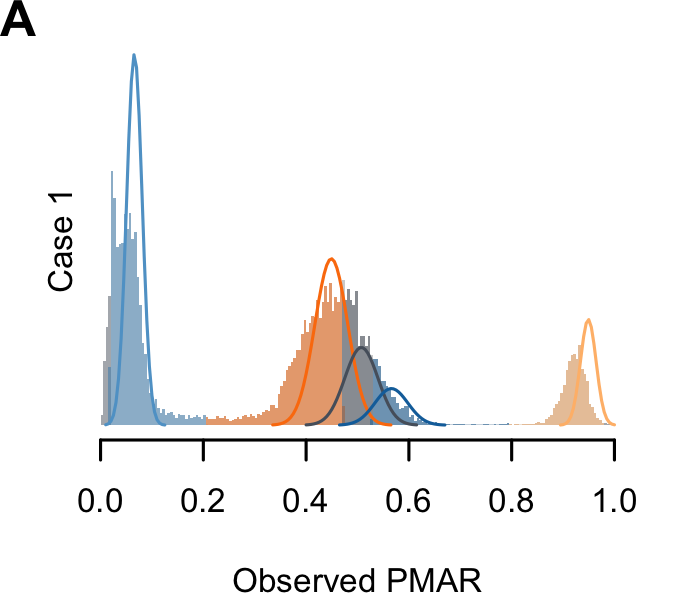
\includegraphics{fig-genoHist-1.pdf}%
  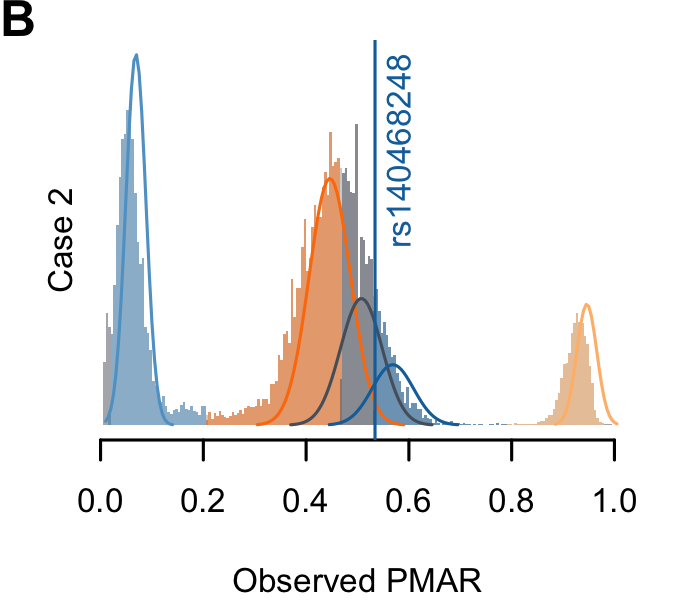
\includegraphics{fig-genoHist-2.pdf}%
  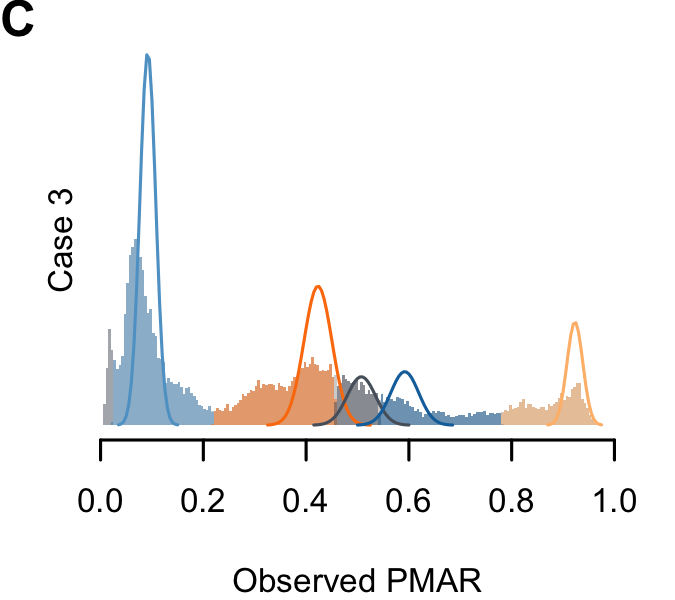
\includegraphics{fig-genoHist-3.pdf}
  
\includegraphics{fig-genoLgnd-1.pdf}
\end{figure}

\newpage
\section{Distribution of fragment lengths}

For Case 3, where we also have direct maternal and fetal exome sequencing, we can attempt to identify maternal and fetal reads in the cell-free exome.
We identify maternal (or fetal) reads by identifying sites with unique heterozygosity in the mother (or fetus), then only interrogating the reads that support the unique allele.

\begin{knitrout}
\definecolor{shadecolor}{rgb}{0.969, 0.969, 0.969}\color{fgcolor}\begin{kframe}
\begin{alltt}
\hlkwd{data}\hlstd{(c3MatFetReads)}
\hlstd{matDen} \hlkwb{<-} \hlkwd{density}\hlstd{(c3MatFetReads[source} \hlopt{==} \hlstr{"maternal"}\hlstd{, isize])}
\hlstd{fetDen} \hlkwb{<-} \hlkwd{density}\hlstd{(c3MatFetReads[source} \hlopt{==} \hlstr{"fetal"}\hlstd{,    isize])}
\hlkwd{par}\hlstd{(}\hlkwc{mar} \hlstd{=} \hlkwd{c}\hlstd{(}\hlnum{4}\hlstd{,} \hlnum{4}\hlstd{,} \hlnum{1}\hlstd{,} \hlnum{1}\hlstd{))}
\hlkwd{plot.new}\hlstd{()}
\hlkwd{plot.window}\hlstd{(}\hlkwc{xlim} \hlstd{=} \hlkwd{range}\hlstd{(}\hlkwd{c}\hlstd{(matDen}\hlopt{$}\hlstd{x, fetDen}\hlopt{$}\hlstd{x)),} \hlkwd{range}\hlstd{(}\hlkwd{c}\hlstd{(matDen}\hlopt{$}\hlstd{y, fetDen}\hlopt{$}\hlstd{y)))}
\hlkwd{lines}\hlstd{(matDen,} \hlkwc{col} \hlstd{=} \hlstr{"darkblue"}\hlstd{,} \hlkwc{lwd} \hlstd{=} \hlnum{2}\hlstd{)}
\hlkwd{lines}\hlstd{(fetDen,} \hlkwc{col} \hlstd{=} \hlstr{"darkorange"}\hlstd{,} \hlkwc{lwd} \hlstd{=}\hlnum{2}\hlstd{)}
\hlkwd{axis}\hlstd{(}\hlkwc{side} \hlstd{=} \hlnum{1}\hlstd{)}
\hlkwd{title}\hlstd{(}\hlkwc{xlab} \hlstd{=} \hlstr{"Fragment length (read-pair insert size)"}\hlstd{,} \hlkwc{ylab} \hlstd{=} \hlstr{"Density"}\hlstd{)}
\hlkwd{addfiglab}\hlstd{(}\hlstr{"A"}\hlstd{,} \hlkwc{cex} \hlstd{=} \hlnum{1.5}\hlstd{)}
\hlstd{matCdf} \hlkwb{<-} \hlkwd{ecdf}\hlstd{(c3MatFetReads[source} \hlopt{==} \hlstr{"maternal"}\hlstd{, isize])}
\hlstd{fetCdf} \hlkwb{<-} \hlkwd{ecdf}\hlstd{(c3MatFetReads[source} \hlopt{==} \hlstr{"fetal"}\hlstd{,    isize])}
\hlkwd{plot.new}\hlstd{()}
\hlstd{xv} \hlkwb{<-} \hlkwd{seq}\hlstd{(}\hlnum{50}\hlstd{,} \hlnum{300}\hlstd{,} \hlnum{1}\hlstd{)}
\hlkwd{plot.window}\hlstd{(}\hlkwc{xlim} \hlstd{=} \hlkwd{range}\hlstd{(xv),} \hlkwc{ylim} \hlstd{=} \hlnum{0}\hlopt{:}\hlnum{1}\hlstd{)}
\hlkwd{points}\hlstd{(}\hlkwc{x} \hlstd{= xv,} \hlkwc{y} \hlstd{=} \hlkwd{matCdf}\hlstd{(xv),} \hlkwc{col} \hlstd{=} \hlstr{"darkblue"}\hlstd{,} \hlkwc{lwd} \hlstd{=} \hlnum{2}\hlstd{,} \hlkwc{type} \hlstd{=} \hlstr{"l"}\hlstd{)}
\hlkwd{points}\hlstd{(}\hlkwc{x} \hlstd{= xv,} \hlkwc{y} \hlstd{=} \hlkwd{fetCdf}\hlstd{(xv),} \hlkwc{col} \hlstd{=} \hlstr{"darkorange"}\hlstd{,} \hlkwc{lwd} \hlstd{=} \hlnum{2}\hlstd{,} \hlkwc{type} \hlstd{=} \hlstr{"l"}\hlstd{)}
\hlkwd{addfiglab}\hlstd{(}\hlstr{"B"}\hlstd{,} \hlkwc{cex} \hlstd{=} \hlnum{1.5}\hlstd{)}
\hlkwd{axis}\hlstd{(}\hlkwc{side} \hlstd{=} \hlnum{1}\hlstd{)}
\hlkwd{axis}\hlstd{(}\hlkwc{side} \hlstd{=} \hlnum{2}\hlstd{)}
\hlkwd{title}\hlstd{(}\hlkwc{xlab} \hlstd{=} \hlstr{"Fragment length (read-pair insert size)"}\hlstd{,}
      \hlkwc{ylab} \hlstd{=} \hlstr{"Cumulative distribution"}\hlstd{)}
\end{alltt}
\end{kframe}
\end{knitrout}

\begin{knitrout}
\definecolor{shadecolor}{rgb}{0.969, 0.969, 0.969}\color{fgcolor}\begin{kframe}
\begin{alltt}
\hlkwd{par}\hlstd{(}\hlkwc{mar} \hlstd{=} \hlkwd{rep}\hlstd{(}\hlnum{0}\hlstd{,} \hlnum{4}\hlstd{))}
\hlkwd{plot.new}\hlstd{()}
\hlkwd{legend}\hlstd{(}\hlkwc{x} \hlstd{=} \hlkwd{grconvertX}\hlstd{(}\hlnum{0.5}\hlstd{,} \hlkwc{from} \hlstd{=} \hlstr{"ndc"}\hlstd{),}
       \hlkwc{y} \hlstd{=} \hlkwd{grconvertY}\hlstd{(}\hlnum{0.5}\hlstd{,} \hlkwc{from} \hlstd{=} \hlstr{"ndc"}\hlstd{),}
       \hlkwc{legend} \hlstd{=} \hlkwd{c}\hlstd{(}\hlstr{"Maternal"}\hlstd{,} \hlstr{"Fetal"}\hlstd{),}
       \hlkwc{horiz} \hlstd{=} \hlnum{TRUE}\hlstd{,}
       \hlkwc{lwd} \hlstd{=} \hlnum{2}\hlstd{,}
       \hlkwc{col} \hlstd{=} \hlkwd{c}\hlstd{(}\hlstr{"darkblue"}\hlstd{,} \hlstr{"darkorange"}\hlstd{),}
       \hlkwc{xjust} \hlstd{=} \hlnum{0.5}\hlstd{,}
       \hlkwc{yjust} \hlstd{=} \hlnum{0.5}\hlstd{,}
       \hlkwc{xpd} \hlstd{=} \hlnum{NA}\hlstd{,}
       \hlkwc{bty} \hlstd{=} \hlstr{"n"}\hlstd{)}
\end{alltt}
\end{kframe}
\end{knitrout}

\begin{figure}
  \centering
  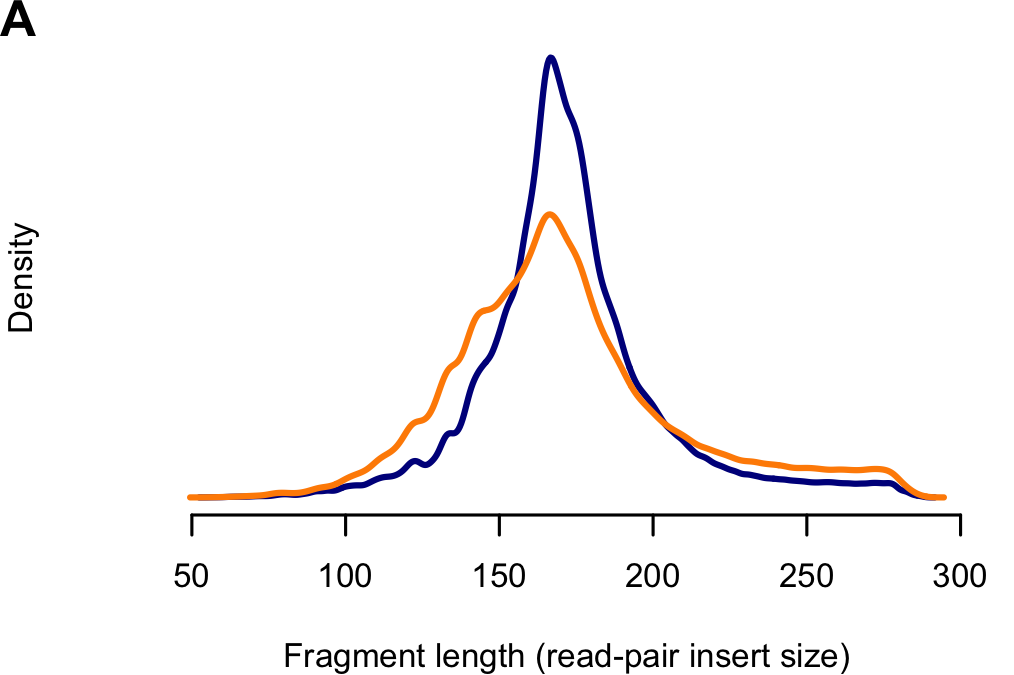
\includegraphics{fig-f34FragLen-1.pdf}%
  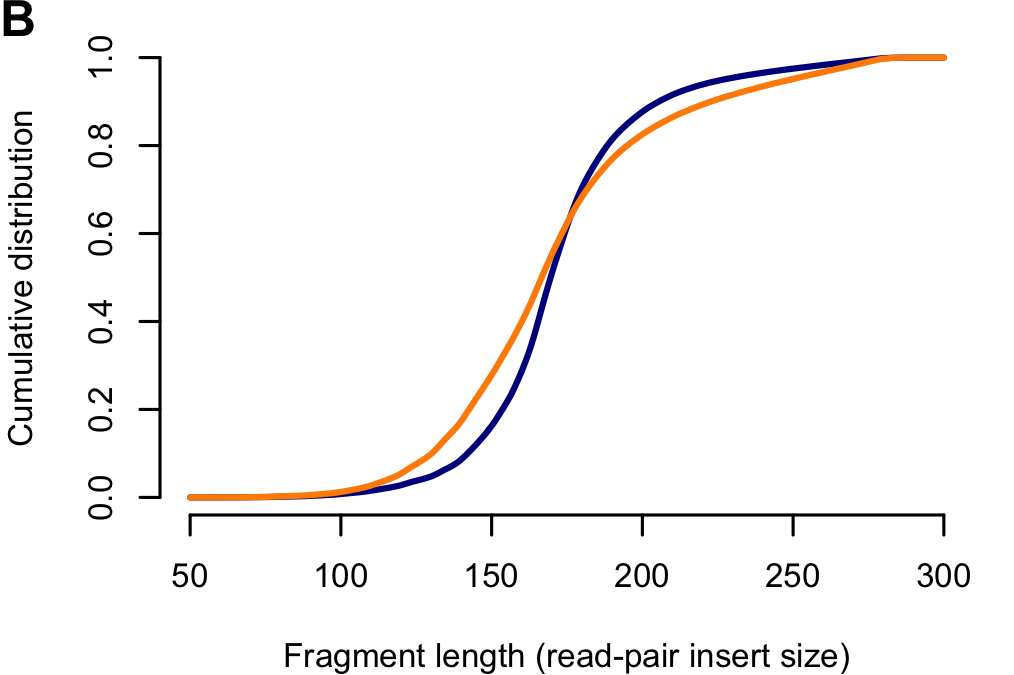
\includegraphics{fig-f34FragLen-2.pdf}
  
\includegraphics{fig-fragLgnd-1.pdf}
\end{figure}

We can also evaluate the distribution of proprtion of fragments with insert sizes less than 140.

\begin{knitrout}
\definecolor{shadecolor}{rgb}{0.969, 0.969, 0.969}\color{fgcolor}\begin{kframe}
\begin{alltt}
\hlstd{gt[ , pmar} \hlkwb{:=} \hlstd{alt}\hlopt{/}\hlstd{(alt} \hlopt{+} \hlstd{ref)]}
\hlstd{gt[ , sratio} \hlkwb{:=} \hlstd{sdep}\hlopt{/}\hlstd{adep]}
\hlstd{pltSratioByPmar} \hlkwb{<-} \hlkwa{function}\hlstd{(}\hlkwc{smpNm}\hlstd{) \{}
  \hlkwd{par}\hlstd{(}\hlkwc{mar} \hlstd{=} \hlkwd{c}\hlstd{(}\hlnum{4}\hlstd{,} \hlnum{4}\hlstd{,} \hlnum{1}\hlstd{,} \hlnum{1}\hlstd{))}
  \hlkwd{with}\hlstd{(gt[gtCall} \hlopt{==} \hlstr{"AAab"} \hlopt{&} \hlstd{smp} \hlopt{==} \hlstd{smpNm], \{}
    \hlkwd{plot}\hlstd{(pmar} \hlopt{~} \hlstd{sratio,}
         \hlkwc{xlab} \hlstd{=} \hlstr{"Proportion of fragments < 140 bp"}\hlstd{,}
         \hlkwc{ylab} \hlstd{=} \hlstr{"PMAR"}\hlstd{,}
         \hlkwc{pch} \hlstd{=} \hlnum{16}\hlstd{,}
         \hlkwc{cex} \hlstd{=} \hlnum{0.5}\hlstd{,}
         \hlkwc{col} \hlstd{=} \hlkwd{col2alpha}\hlstd{(}\hlstr{'darkgray'}\hlstd{),}
         \hlkwc{bty} \hlstd{=} \hlstr{"n"}\hlstd{)}
  \hlstd{\})}
  \hlkwd{with}\hlstd{(gt[gtCall} \hlopt{==} \hlstr{"AAab"} \hlopt{&} \hlstd{smp} \hlopt{==} \hlstd{smpNm], \{}
    \hlkwd{contour}\hlstd{(}\hlkwd{kde2d}\hlstd{(}\hlkwc{x} \hlstd{= sratio,} \hlkwc{y} \hlstd{= pmar,} \hlkwc{n} \hlstd{=} \hlnum{500}\hlstd{),}
            \hlkwc{nlevels} \hlstd{=} \hlnum{25}\hlstd{,}
            \hlkwc{add} \hlstd{=} \hlnum{TRUE}\hlstd{,}
            \hlkwc{drawlabels} \hlstd{=} \hlnum{FALSE}\hlstd{,}
            \hlkwc{col} \hlstd{=} \hlstr{"darkblue"}\hlstd{)}
  \hlstd{\})}
\hlstd{\}}
\hlkwd{pltSratioByPmar}\hlstd{(}\hlstr{"S1"}\hlstd{)}
\hlkwd{addfiglab}\hlstd{(}\hlstr{"A"}\hlstd{,} \hlkwc{cex} \hlstd{=} \hlnum{1.5}\hlstd{)}
\hlkwd{pltSratioByPmar}\hlstd{(}\hlstr{"S2"}\hlstd{)}
\hlkwd{addfiglab}\hlstd{(}\hlstr{"B"}\hlstd{,} \hlkwc{cex} \hlstd{=} \hlnum{1.5}\hlstd{)}
\hlkwd{pltSratioByPmar}\hlstd{(}\hlstr{"FES-0034-4"}\hlstd{)}
\hlkwd{addfiglab}\hlstd{(}\hlstr{"C"}\hlstd{,} \hlkwc{cex} \hlstd{=} \hlnum{1.5}\hlstd{)}
\end{alltt}
\end{kframe}
\end{knitrout}

\begin{figure}
  \centering
  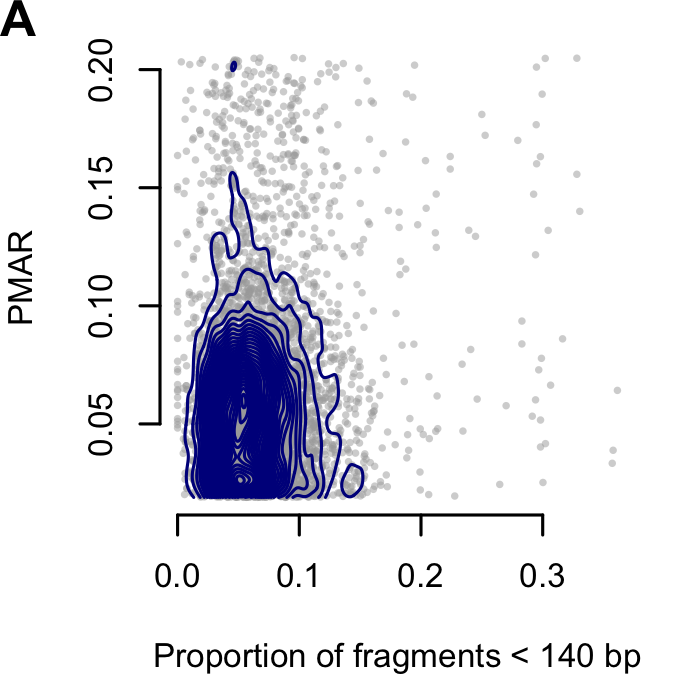
\includegraphics{fig-pmarBySratio-1.pdf}%
  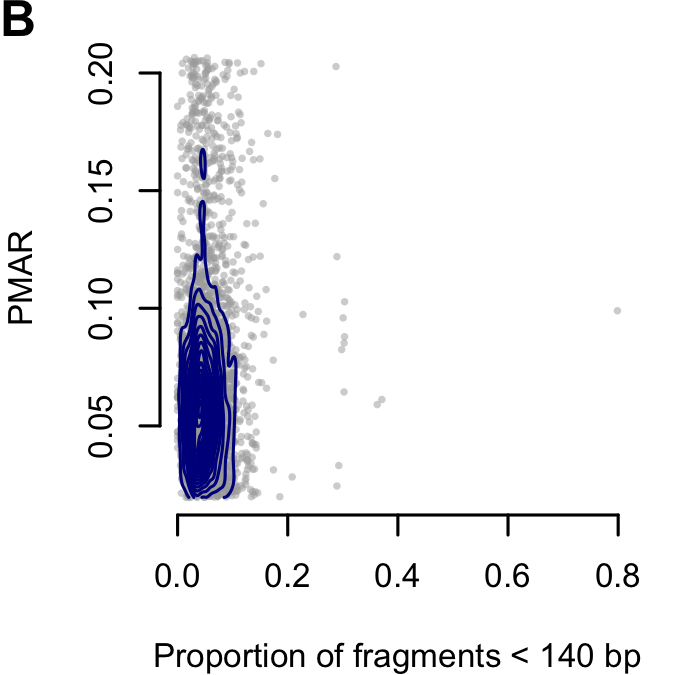
\includegraphics{fig-pmarBySratio-2.pdf}%
  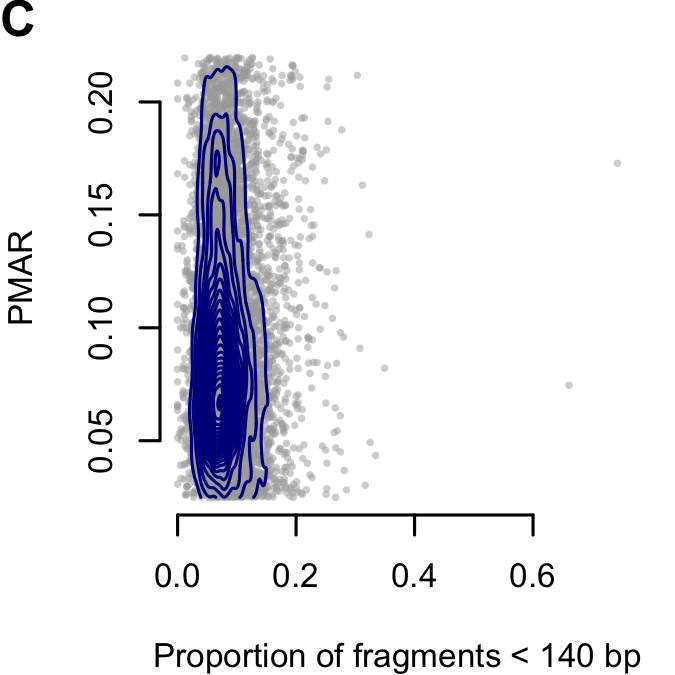
\includegraphics{fig-pmarBySratio-3.pdf}
\end{figure}

\newpage
\section{Calculate call concordance between cell-free and direct for Case 3}

\begin{knitrout}
\definecolor{shadecolor}{rgb}{0.969, 0.969, 0.969}\color{fgcolor}\begin{kframe}
\begin{alltt}
\hlstd{c3} \hlkwb{<-} \hlstd{gt[(smp} \hlopt{==} \hlstr{"FES-0034-0"} \hlopt{&} \hlstd{udep} \hlopt{>} \hlnum{30} \hlopt{&} \hlstd{gt} \hlopt \hlkwd{c}\hlstd{(}\hlstr{"0/0"}\hlstd{,} \hlstr{"0/1"}\hlstd{,} \hlstr{"1/1"}\hlstd{))} \hlopt{|}
           \hlstd{(smp} \hlopt{==} \hlstr{"FES-0034-1"} \hlopt{&} \hlstd{udep} \hlopt{>} \hlnum{30} \hlopt{&} \hlstd{gt} \hlopt \hlkwd{c}\hlstd{(}\hlstr{"0/0"}\hlstd{,} \hlstr{"0/1"}\hlstd{,} \hlstr{"1/1"}\hlstd{))} \hlopt{|}
           \hlstd{(use} \hlopt{&} \hlstd{smp} \hlopt{==} \hlstr{"FES-0034-4"}\hlstd{)]}
\hlstd{c3[ , mrg} \hlkwb{:=} \hlkwd{substr}\hlstd{(gtCall,} \hlnum{3}\hlstd{,} \hlnum{4}\hlstd{)]}
\hlstd{c3[ , mrg} \hlkwb{:=} \hlkwd{c}\hlstd{(}\hlstr{"0/0"}\hlstd{,} \hlstr{"0/1"}\hlstd{,} \hlstr{"1/1"}\hlstd{)[}\hlkwd{match}\hlstd{(mrg,} \hlkwd{c}\hlstd{(}\hlstr{"aa"}\hlstd{,} \hlstr{"ab"}\hlstd{,} \hlstr{"bb"}\hlstd{))]]}
\hlstd{c3[}\hlkwd{is.na}\hlstd{(gtCall), mrg} \hlkwb{:=} \hlstd{gt]}
\hlstd{c3} \hlkwb{<-} \hlkwd{dcast}\hlstd{(c3, varid} \hlopt{~} \hlstd{smp,} \hlkwc{value.var} \hlstd{=} \hlstr{"mrg"}\hlstd{)}
\hlkwd{setnames}\hlstd{(c3,} \hlkwd{c}\hlstd{(}\hlstr{"varid"}\hlstd{,} \hlstr{"fet"}\hlstd{,} \hlstr{"mat"}\hlstd{,} \hlstr{"cff"}\hlstd{))}
\hlstd{c3} \hlkwb{<-} \hlstd{c3[ , .N,} \hlkwc{by} \hlstd{=} \hlkwd{.}\hlstd{(mat, fet, cff)]}
\hlstd{c3[}\hlopt{!}\hlkwd{is.na}\hlstd{(mat)} \hlopt{& !}\hlkwd{is.na}\hlstd{(fet)} \hlopt{& !}\hlkwd{is.na}\hlstd{(cff), ][}\hlkwd{order}\hlstd{(mat, fet, cff)]}
\end{alltt}
\begin{verbatim}
##     mat fet cff    N
##  1: 0/0 0/0 0/0  468
##  2: 0/0 0/0 0/1 1159
##  3: 0/0 0/1 0/0   64
##  4: 0/0 0/1 0/1  352
##  5: 0/0 1/1 0/0    1
##  6: 0/0 1/1 0/1    2
##  7: 0/1 0/0 0/0  387
##  8: 0/1 0/0 0/1  107
##  9: 0/1 0/0 1/1    6
## 10: 0/1 0/1 0/0 3072
## 11: 0/1 0/1 0/1 1967
## 12: 0/1 0/1 1/1  713
## 13: 0/1 1/1 0/0   68
## 14: 0/1 1/1 0/1  458
## 15: 0/1 1/1 1/1 1291
## 16: 1/1 0/0 0/1    1
## 17: 1/1 0/0 1/1    2
## 18: 1/1 0/1 0/0    3
## 19: 1/1 0/1 0/1 1308
## 20: 1/1 0/1 1/1  648
## 21: 1/1 1/1 0/1 1601
## 22: 1/1 1/1 1/1   23
##     mat fet cff    N
\end{verbatim}
\begin{alltt}
\hlcom{## call by call matrix, cell-free calls in columns, fetal in rows}
\hlkwd{dcast}\hlstd{(c3[}\hlopt{!}\hlkwd{is.na}\hlstd{(cff)} \hlopt{& !}\hlkwd{is.na}\hlstd{(fet)], fet} \hlopt{~} \hlstd{cff,}
      \hlkwc{value.var} \hlstd{=} \hlstr{"N"}\hlstd{,} \hlkwc{fun.aggregate} \hlstd{= sum)}
\end{alltt}
\begin{verbatim}
##    fet  0/0  0/1  1/1
## 1: 0/0 1063 1857    9
## 2: 0/1 3598 7079 1454
## 3: 1/1   76 2197 1391
\end{verbatim}
\end{kframe}
\end{knitrout}



\newpage
\section{Binomial distribution bounds}

\begin{knitrout}
\definecolor{shadecolor}{rgb}{0.969, 0.969, 0.969}\color{fgcolor}\begin{kframe}
\begin{alltt}
\hlkwd{pltExpMAF}\hlstd{(}\hlnum{500}\hlstd{)}
\hlkwd{addfiglab}\hlstd{(}\hlstr{"A"}\hlstd{,} \hlkwc{cex} \hlstd{=} \hlnum{1.5}\hlstd{)}
\hlkwd{pltMissclass}\hlstd{()}
\hlkwd{addfiglab}\hlstd{(}\hlstr{"B"}\hlstd{,} \hlkwc{cex} \hlstd{=} \hlnum{1.5}\hlstd{)}
\end{alltt}
\end{kframe}
\end{knitrout}

\begin{figure}
  \centering
  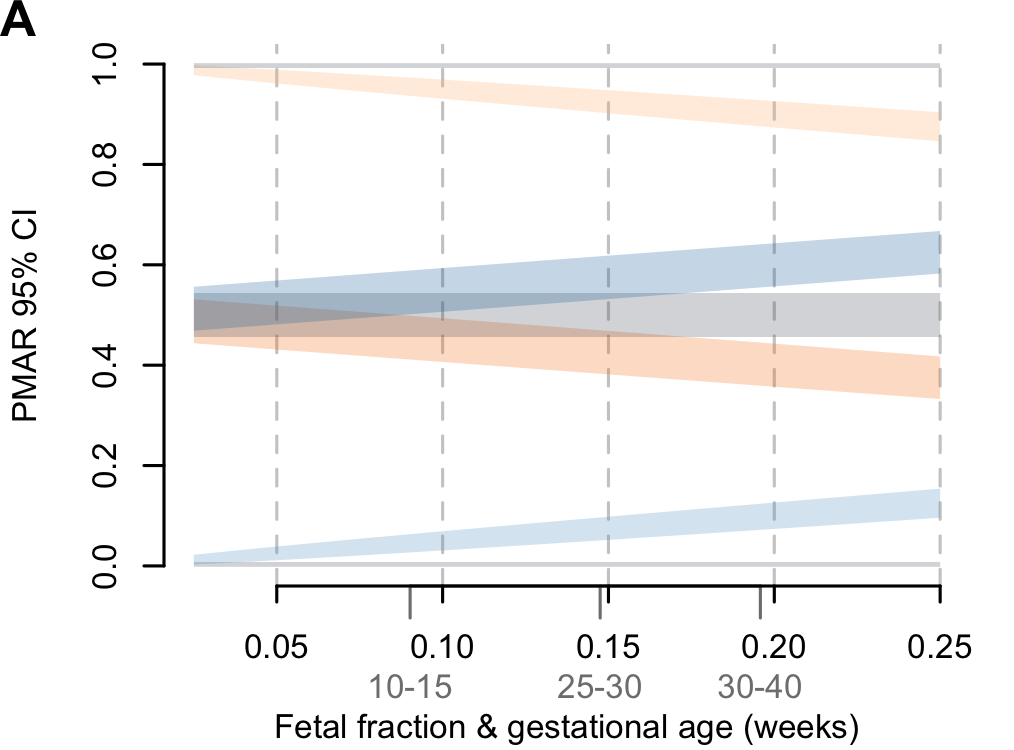
\includegraphics{fig-binDist-1.pdf}%
  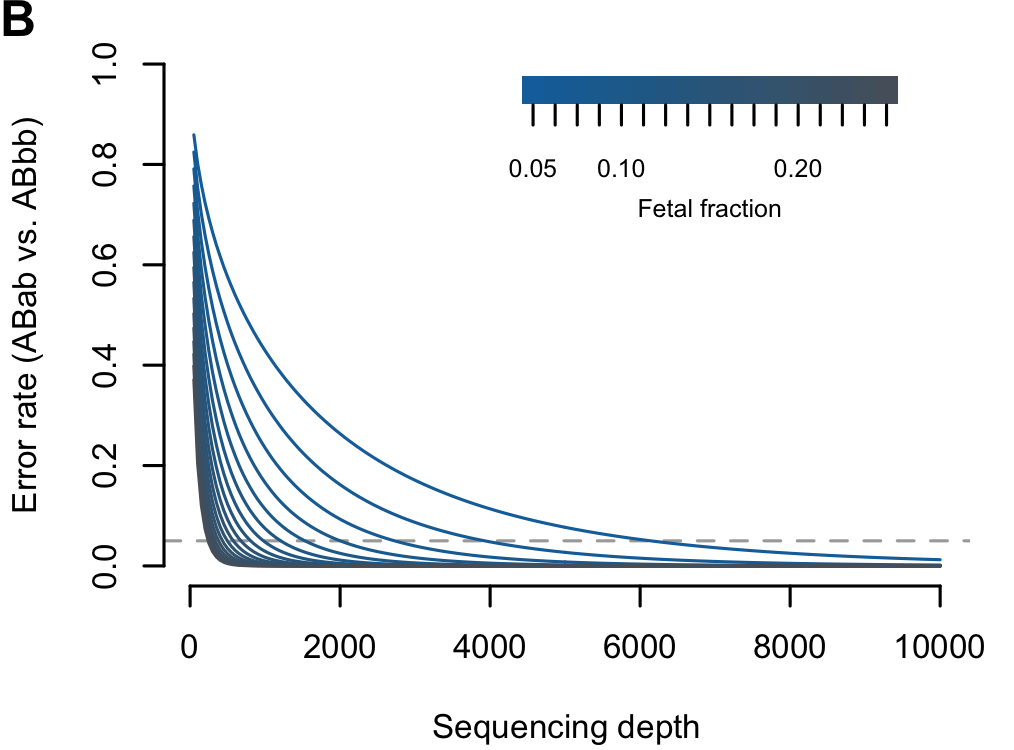
\includegraphics{fig-binDist-2.pdf}
  
\includegraphics{fig-genoLgnd-1.pdf}
\end{figure}

\section{Snakemake file}

Note, Snakemake file and all accessory files contained within the filer2020B package `inst' directory.

\begin{knitrout}
\definecolor{shadecolor}{rgb}{0.969, 0.969, 0.969}\color{fgcolor}\begin{kframe}
\begin{verbatim}
configfile: "config.yaml"
shell.prefix('export TMPDIR=%s;'%(config['temp_dir']))

sampleRuns = dict()
fastqs = []
cases = []
samples = []
for (c,s,r,f) in zip(*glob_wildcards('inputs/{case}/{sample}/{runId}/{fastqBase}.fastq.gz')):
    sampleRuns.setdefault(c, {}).setdefault(s, {}).setdefault(r, []).append(f)
    fastqs.append('fastqc/%s/%s/%s_fastqc.zip'%(s,r,f))
    samples.append(s)
    cases.append(c)
    
def getCase(sample):
    for c in sampleRuns:
        if sample in sampleRuns[c]:
            return(c)

rule all:
    input:
        fastqs,
        #expand('normed/{case}.norm.vcf.gz', case = cases),
        #expand('depth/{sample}.nofilt.depth', sample = samples),
        expand('pileup/{sample}.pileup', sample = samples),
        expand('unzip/{sample}.vcf.gz.tbi', sample = samples),
        expand('norm/{sample}.normSnp.vcf.gz.tbi', sample = samples),
        expand('adep/{sample}.adep', sample = samples),
        expand('fdist/{sample}.fdist', sample = samples),
        expand('final/{sample}.final', sample = samples),
        expand('recal/{sample}.recal.bam.alignMetrics', sample = samples),
        expand('recal/{sample}.recal.bam.flagstat', sample = samples),
        expand('keep/{sample}.keep.bai', sample = samples),
        expand('keep/{sample}.keep.bam.alignMetrics', sample = samples),

rule fastqc:
    input:
        lambda wildcards: 
            expand("inputs/{case}/{sample}/{runId}/{stem}.fastq.gz", \
                   case = getCase(wildcards.sample), \
                   sample = wildcards.sample, \
                   runId = wildcards.runId, \
                   stem = sampleRuns[getCase(wildcards.sample)][wildcards.sample][wildcards.runId])
    output:
        html = "fastqc/{sample}/{runId}/{stem}.html",
        zip = "fastqc/{sample}/{runId}/{stem}_fastqc.zip"
    params: ""
    wrapper:
        "0.35.1/bio/fastqc"

rule bwamem:
    input:
        reads = lambda wildcards: 
            expand('inputs/{case}/{sample}/{runId}/{stem}.fastq.gz', \
                   case = getCase(wildcards.sample), \
                   sample = wildcards.sample, \
                   runId = wildcards.runId, \
                   stem = sampleRuns[getCase(wildcards.sample)][wildcards.sample][wildcards.runId])
    output:
        temp("mapped/{sample}.{runId}.bam")
    log:
        "logs/bwa_mem/{sample}.{runId}.log"
    params:
        index = config['genome_fasta'],
        extra = r"-R '@RG\tID:{sample}_{runId}\tSM:{sample}\tPL:Illumina\tCN:UNC'",
        sort = "picard",
        sort_order = "queryname",
        sort_extra = 'TMP_DIR="%s"'%config['temp_dir']
    threads: 8
    wrapper:
        "0.35.1/bio/bwa/mem"

rule mergeRuns:
    input: lambda wildcards: 
        expand('mapped/{sample}.{runId}.bam', \
               sample = wildcards.sample, \
               runId = sampleRuns[getCase(wildcards.sample)][wildcards.sample])
    output: temp("merged/{sample}.bam")
    params: "-n"
    threads: 8
    wrapper:
        "0.35.1/bio/samtools/merge"

rule markdup:
    input:
        "merged/{sample}.bam"
    output:
        bam = temp("markdup/{sample}.markdup.bam"),
        metrics = "markdup/{sample}.markdup.markdupMetrics"
    log:
        "logs/picard/markdup/{sample}.markdup.log"
    params:
        "REMOVE_DUPLICATES=false",
        "ASSUME_SORT_ORDER=queryname",
        "CREATE_INDEX=false",
        "TAGGING_POLICY=All",
        'TMP_DIR="%s"'%config['temp_dir']
    wrapper:
        "0.35.1/bio/picard/markduplicates"

rule sort:
    input: "markdup/{sample}.markdup.bam"
    output: temp("sorted/{sample}.sorted.markdup.bam")
    params: "-m 2G"
    threads: 8
    wrapper:
        "0.35.1/bio/samtools/sort"

rule indexSorted:
    input: "sorted/{sample}.sorted.markdup.bam"
    output: temp("sorted/{sample}.sorted.markdup.bam.bai")
    wrapper:
        "0.35.1/bio/samtools/index"
        
rule gatkBqsr:
    input:
        bam = "sorted/{sample}.sorted.markdup.bam",
        ref = config['genome_fasta'],
        known = config['known_snp'],
        baiPlaceholder = "sorted/{sample}.sorted.markdup.bam.bai"
    output:
        bam = "recal/{sample}.recal.bam",
        bai = "recal/{sample}.recal.bai"
    log:
        "logs/gatk/bqsr/{sample}.log"
    params:
        extra = "",  # optional
        java_opts = "-Xmx20G -XX:ParallelGCThreads=8", # optional
    threads: 8
    wrapper:
        "0.49.0/bio/gatk/baserecalibrator"

rule alignMetrics:
    input:
        bam = "recal/{sample}.recal.bam",
        ref = config['genome_fasta']
    output:
        "recal/{sample}.recal.bam.alignMetrics"
    log:
        "logs/picard/collectalignmentsummarymetrics/{sample}.log"
    wrapper:
        "0.35.1/bio/picard/collectalignmentsummarymetrics"

rule flagstat:
    input: "recal/{sample}.recal.bam"
    output: "recal/{sample}.recal.bam.flagstat"
    wrapper:
        "0.35.1/bio/samtools/flagstat"

rule preFiltDep:
    input: 
        bam = "recal/{sample}.recal.bam",
        bai = "recal/{sample}.recal.bai",
    output: "depth/{sample}.nofilt.depth"
    conda: "envs/depth.yaml"
    shell:
        "bedtools genomecov -dz -pc -ibam {input.bam} > {output}"

rule subsetPairs:
    input: 
        bam = "recal/{sample}.recal.bam",
        bed = config['overlap_exome'],
        bai = "recal/{sample}.recal.bai",
    output: temp("pairs/{sample}.sortedPairs.bam")
    conda: "envs/subsetPairs.yaml"
    threads: 8
    shell:
        "java -jar {config[viewPairs]} --bed {input.bed} "
        "--samoutputformat BAM {input.bam} | "
        "samtools view -F 3072 -f 2 -b | "
        "picard SortSam SO=queryname I=/dev/stdin O={output}"

rule keep:
    input: "pairs/{sample}.sortedPairs.bam"
    output: 
        bam = "keep/{sample}.keep.bam",
        bai = "keep/{sample}.keep.bai"
    conda: "envs/keep.yaml"
    shell:
        "java -jar {config[samjdk]} --pair "
        "-f scripts/highQualMap.java "
        "--samoutputformat BAM {input} | "
        "picard SortSam SO=coordinate CREATE_INDEX=true "
        "I=/dev/stdin O={output.bam} "
        "TMP_DIR={config[temp_dir]} "

rule alignMetricsKeep:
    input:
        bam = "keep/{sample}.keep.bam",
        ref = config['genome_fasta']
    output:
        "keep/{sample}.keep.bam.alignMetrics"
    log:
        "logs/picard/collectalignmentsummarymetrics/{sample}.keep.log"
    wrapper:
        "0.35.1/bio/picard/collectalignmentsummarymetrics"

rule depthAll:
    input:
        bam = "keep/{sample}.keep.bam",
        bai = "keep/{sample}.keep.bai"
    output: "depth/{sample}.all.depth"
    conda: "envs/depth.yaml"
    shell:
        "bedtools genomecov -dz -pc -ibam {input.bam} > {output}"

rule depthFetTemp:
    input:
        bam = "keep/{sample}.keep.bam",
        bai = "keep/{sample}.keep.bai"
    output: temp("depth/{sample}.fet.depth.bam")
    conda: "envs/depth.yaml"
    shell:
        "java -jar {config[samjdk]} "
        "-e ' "
        "int is = record.getInferredInsertSize(); "
        "if (is < 0) is = is * -1; return is < 140; "
        " ' "
        "--samoutputformat BAM {input.bam} > {output} "

rule depthFet:
    input: "depth/{sample}.fet.depth.bam",
    output: "depth/{sample}.fet.depth"
    conda: "envs/depth.yaml"
    shell:
        "bedtools genomecov -dz -pc -ibam {input} > {output}"

rule depthMatTemp:
    input:
        bam = "keep/{sample}.keep.bam",
        bai = "keep/{sample}.keep.bai"
    output: temp("depth/{sample}.mat.depth.bam")
    conda: "envs/depth.yaml"
    shell:
        "java -jar {config[samjdk]} "
        "-e ' "
        "int is = record.getInferredInsertSize(); "
        "if (is < 0) is = is * -1; return is > 166 && is < 1000; "
        " ' "
        "--samoutputformat BAM {input.bam} > {output} "

rule depthMat:
    input: "depth/{sample}.mat.depth.bam",
    output: "depth/{sample}.mat.depth"
    conda: "envs/depth.yaml"
    shell:
        "bedtools genomecov -dz -pc -ibam {input} > {output}"

rule mpileup:
    input: 
        bam = "keep/{sample}.keep.bam",
        ref = config['genome_fasta'],
        tgt = config['overlap_exome'],
    output: "pileup/{sample}.pileup"
    conda: "envs/samtools.yaml"
    shell:
        "samtools mpileup -aa -f {input.ref} -d 100000 "
        "--positions {input.tgt} -Q 20 {input.bam} > "
        "{output} "

rule alleleDep:
    input: 
        bam = "keep/{sample}.keep.bam",
        ref = config['genome_fasta'],
        tgt = config['overlap_exome'],
    output: "calls/{sample}.bcf"
    conda: "envs/bcftools.yaml"
    shell:
        "bcftools mpileup -f {input.ref} -a AD -Q 20 -d 50000 "
        "-R {input.tgt} {input.bam} | bcftools call -m -A "
        "-f GQ,GP -O b -o {output} "

## Removes all sites without an alternate allele; could consider using
## -V indels to only include snps but retain all sites in the exome
rule normAndSubsetCalls:
    input: "calls/{sample}.bcf"
    output: "norm/{sample}.normSnp.vcf.gz"
    conda: "envs/bcftools.yaml"
    shell:
        "bcftools norm -N -O u -m - {input} | "
        "bcftools view -v snps -O z -o {output} "

rule indexNormBcf:
    input: "norm/{sample}.normSnp.vcf.gz"
    output: "norm/{sample}.normSnp.vcf.gz.tbi"
    conda: "envs/bcftools.yaml"
    shell: "bcftools index --tbi {input} -o {output} "
    
rule getFragDist:
    input: 
        adep = "depth/{sample}.all.depth",
        fdep = "depth/{sample}.fet.depth",
        mdep = "depth/{sample}.mat.depth",
        tgt = config['overlap_exome'],
    output: "fdist/{sample}.fdist"
    conda: "envs/r.yaml"
    shell: 
        "scripts/getFragDist.R -a {input.adep} -l {input.mdep} "
        "-s {input.fdep} -r {input.tgt} -o {output}"

rule getAlleleDep:
    input: "norm/{sample}.normSnp.vcf.gz"
    output: "adep/{sample}.adep"
    conda: "envs/r.yaml"
    shell: "scripts/getAlleleCounts.R -v {input} -o {output}"

rule combineAdepFdist:
    input:
        adep = "adep/{sample}.adep",
        fdst = "fdist/{sample}.fdist"
    output: "final/{sample}.final"
    params: 
        tdep = 0,
        mdep = 0,
    conda: "envs/r.yaml"
    shell:
        "scripts/getAdepFdist.R -a {input.adep} -f {input.fdst} "
        "-t {params.tdep} -m {params.mdep} -o {output} "

rule freebayes:
    input:
        ref = config['genome_fasta'],
        samples = lambda wildcards: 
            expand('keep/{sample}.keep.bam', \
                   case = wildcards.case, \
                   sample = sampleRuns[wildcards.case]),
        bai = lambda wildcards: 
            expand('keep/{sample}.keep.bai', \
                   case = wildcards.case, \
                   sample = sampleRuns[wildcards.case]),
        #cnvMap = config['samplePloidy'], also use --pooled-discrete
        targets = config['overlap_exome'],
    output:
        temp("calls/{case}.vcf")
    log:
        "logs/freebayes/{case}.log"
    params:
        extra = "--genotype-qualities \
                 --strict-vcf \
                 --min-alternate-count 5 \
                 --standard-filters \
                 --report-genotype-likelihood-max \
                 --use-mapping-quality",
        chunksize = 100000,
    threads: 8
    conda: "envs/freebayes.yaml"
    shell:
        "(" 
        "freebayes-parallel " 
        "<(fasta_generate_regions.py {input.ref}.fai {params.chunksize}) "
        "{threads} "
        "-f {input.ref} "
        "--targets {input.targets} {params.extra} " 
        "{input.samples} > {output[0]}"
        ") "
        " > {log} 2>&1"

rule compressVcf:
    input: "calls/{stem}.vcf"
    output: temp("calls/{stem}.vcf.gz")
    wrapper: "0.36.0/bio/vcf/compress"

rule normVcf:
    input: "calls/{stem}.vcf.gz"
    output: "normed/{stem}.norm.vcf.gz"
    params: "-m - -O z"
    wrapper: "0.44.2/bio/bcftools/norm"
\end{verbatim}
\end{kframe}
\end{knitrout}

\section{Script to produce package data}

\begin{knitrout}
\definecolor{shadecolor}{rgb}{0.969, 0.969, 0.969}\color{fgcolor}\begin{kframe}
\begin{alltt}
\hlkwd{library}\hlstd{(data.table)}
\hlstd{wd} \hlkwb{<-} \hlkwd{getwd}\hlstd{()} \hlcom{## Snakemake directory}

\hlstd{sampleMeta} \hlkwb{<-} \hlkwd{data.table}\hlstd{(}\hlkwc{smp} \hlstd{=} \hlkwd{c}\hlstd{(}\hlstr{"S1"}\hlstd{,} \hlstr{"S2"}\hlstd{,} \hlkwd{sprintf}\hlstd{(}\hlstr{"FES-0034-%d"}\hlstd{,} \hlkwd{c}\hlstd{(}\hlnum{0}\hlopt{:}\hlnum{2}\hlstd{,} \hlnum{4}\hlstd{))))}
\hlstd{sampleMeta[ , case} \hlkwb{:=} \hlkwd{c}\hlstd{(}\hlnum{1}\hlstd{,} \hlnum{2}\hlstd{,} \hlkwd{rep}\hlstd{(}\hlnum{3}\hlstd{,} \hlnum{4}\hlstd{))]}
\hlstd{sampleMeta[ ,}
            \hlstd{source} \hlkwb{:=} \hlkwd{c}\hlstd{(}\hlstr{"cell-free"}\hlstd{,} \hlstr{"cell-free"}\hlstd{,} \hlstr{"newborn"}\hlstd{,} \hlstr{"maternal"}\hlstd{,}
                        \hlstr{"paternal"}\hlstd{,} \hlstr{"cell-free"}\hlstd{)]}
\hlkwd{save}\hlstd{(sampleMeta,} \hlkwc{file} \hlstd{=} \hlkwd{file.path}\hlstd{(wd,} \hlstr{"forLetter"}\hlstd{,} \hlstr{"sampleMeta.RData"}\hlstd{))}

\hlcom{##----------------------------------------------------------------------------##}
\hlcom{## readSmry}
\hlcom{##----------------------------------------------------------------------------##}

\hlcom{## Read in markdup files}
\hlstd{mdFls} \hlkwb{<-} \hlkwd{list.files}\hlstd{(}\hlkwd{file.path}\hlstd{(wd,} \hlstr{"markdup"}\hlstd{),} \hlkwc{full.names} \hlstd{=} \hlnum{TRUE}\hlstd{)}
\hlstd{readMarkDup} \hlkwb{<-} \hlkwa{function}\hlstd{(}\hlkwc{f}\hlstd{) \{}
  \hlstd{d} \hlkwb{<-} \hlkwd{as.data.table}\hlstd{(}\hlkwd{read.table}\hlstd{(f,} \hlkwc{nrows} \hlstd{=} \hlnum{1}\hlstd{,} \hlkwc{header} \hlstd{=} \hlnum{TRUE}\hlstd{))}
  \hlstd{d[ , f} \hlkwb{:=} \hlkwd{basename}\hlstd{(f)]}
  \hlstd{d[]}
\hlstd{\}}
\hlstd{md} \hlkwb{<-} \hlkwd{rbindlist}\hlstd{(}\hlkwd{lapply}\hlstd{(mdFls, readMarkDup))}
\hlstd{md[ , smp} \hlkwb{:=} \hlkwd{sub}\hlstd{(}\hlstr{".markdup.+$"}\hlstd{,} \hlstr{""}\hlstd{, f)]}

\hlcom{## Read in align metrics files}
\hlstd{amFls} \hlkwb{<-} \hlkwd{Sys.glob}\hlstd{(}\hlkwd{file.path}\hlstd{(wd,} \hlstr{"*"}\hlstd{,} \hlstr{"*.alignMetrics"}\hlstd{))}
\hlstd{readAlign} \hlkwb{<-} \hlkwa{function}\hlstd{(}\hlkwc{f}\hlstd{) \{}
  \hlstd{d} \hlkwb{<-} \hlkwd{fread}\hlstd{(f)}
  \hlstd{d[ , f} \hlkwb{:=} \hlkwd{basename}\hlstd{(f)]}
  \hlstd{d[]}
\hlstd{\}}
\hlstd{am} \hlkwb{<-} \hlkwd{rbindlist}\hlstd{(}\hlkwd{lapply}\hlstd{(amFls, readAlign))}
\hlstd{am[ , smp} \hlkwb{:=} \hlkwd{sub}\hlstd{(}\hlstr{".keep.+$|.recal.+$"}\hlstd{,} \hlstr{""}\hlstd{, f)]}
\hlstd{am[ , set} \hlkwb{:=} \hlkwd{ifelse}\hlstd{(}\hlkwd{grepl}\hlstd{(}\hlstr{"recal"}\hlstd{, f),} \hlstr{"recal"}\hlstd{,} \hlstr{"keep"}\hlstd{)]}

\hlcom{## Create summary object}
\hlstd{rp} \hlkwb{<-} \hlstd{md[ ,} \hlkwd{.}\hlstd{(smp,} \hlkwc{ttl} \hlstd{= READ_PAIRS_EXAMINED}\hlopt{*}\hlnum{2}\hlstd{,} \hlkwc{pctDup} \hlstd{= PERCENT_DUPLICATION)]}
\hlstd{rp[ , dup} \hlkwb{:=} \hlstd{ttl}\hlopt{*}\hlstd{pctDup]}
\hlkwd{setkey}\hlstd{(rp, smp)}
\hlkwd{setkey}\hlstd{(am, smp)}
\hlstd{rp} \hlkwb{<-} \hlstd{am[set} \hlopt{==} \hlstr{"keep"} \hlopt{&} \hlstd{CATEGORY} \hlopt{==} \hlstr{"PAIR"}\hlstd{,} \hlkwd{.}\hlstd{(smp,} \hlkwc{keep} \hlstd{= TOTAL_READS)][rp]}
\hlstd{rp[ , pctFlt} \hlkwb{:=} \hlstd{(ttl} \hlopt{-} \hlstd{dup} \hlopt{-} \hlstd{keep)}\hlopt{/}\hlstd{ttl}\hlopt{*}\hlnum{100}\hlstd{]}
\hlstd{rp[ , pctDup} \hlkwb{:=} \hlstd{pctDup} \hlopt{*}\hlnum{100}\hlstd{]}

\hlstd{readSmry} \hlkwb{<-} \hlkwd{list}\hlstd{(}\hlkwc{summary} \hlstd{= rp,}
                 \hlkwc{markDuplicates} \hlstd{= md,}
                 \hlkwc{alignMetrics} \hlstd{= am)}

\hlkwd{save}\hlstd{(readSmry,} \hlkwc{file} \hlstd{=} \hlkwd{file.path}\hlstd{(wd,} \hlstr{"forLetter"}\hlstd{,} \hlstr{"readSmry.RData"}\hlstd{))}

\hlcom{##----------------------------------------------------------------------------##}
\hlcom{## gt}
\hlcom{##----------------------------------------------------------------------------##}

\hlstd{gtFls} \hlkwb{<-} \hlkwd{list.files}\hlstd{(}\hlkwd{file.path}\hlstd{(wd,} \hlstr{"final"}\hlstd{),} \hlkwc{full.names} \hlstd{=} \hlnum{TRUE}\hlstd{)}
\hlstd{rdFinal} \hlkwb{<-} \hlkwa{function}\hlstd{(}\hlkwc{fl}\hlstd{) \{}
  \hlstd{x} \hlkwb{<-} \hlkwd{readRDS}\hlstd{(fl)}
  \hlstd{x[ , smp} \hlkwb{:=} \hlkwd{sub}\hlstd{(}\hlstr{".final"}\hlstd{,} \hlstr{""}\hlstd{,} \hlkwd{basename}\hlstd{(fl))]}
\hlstd{\}}

\hlstd{gt} \hlkwb{<-} \hlkwd{rbindlist}\hlstd{(}\hlkwd{lapply}\hlstd{(gtFls, rdFinal))}
\hlstd{gt} \hlkwb{<-} \hlstd{gt[}\hlopt{!}\hlkwd{is.na}\hlstd{(adep)]}
\hlstd{gt[ ,} \hlkwd{c}\hlstd{(}\hlstr{"chr"}\hlstd{,} \hlstr{"var"}\hlstd{)} \hlkwb{:=} \hlkwd{tstrsplit}\hlstd{(id,} \hlstr{":"}\hlstd{)]}
\hlstd{gt[ , chr} \hlkwb{:=} \hlkwd{as.integer}\hlstd{(}\hlkwd{gsub}\hlstd{(}\hlstr{"^NC_0+|[:.:][0-9][0-9]$"}\hlstd{,} \hlstr{""}\hlstd{, chr))]}
\hlstd{gt[ ,} \hlkwd{c}\hlstd{(}\hlstr{"pos"}\hlstd{,} \hlstr{"bp"}\hlstd{)} \hlkwb{:=} \hlkwd{tstrsplit}\hlstd{(var,} \hlstr{"_"}\hlstd{,} \hlkwc{type.convert} \hlstd{=} \hlnum{TRUE}\hlstd{)]}
\hlstd{gt[ , pos} \hlkwb{:=} \hlkwd{round}\hlstd{(pos,} \hlopt{-}\hlnum{4}\hlstd{)]}
\hlstd{gt[ ,} \hlkwd{c}\hlstd{(}\hlstr{"var"}\hlstd{,} \hlstr{"bp"}\hlstd{)} \hlkwb{:=} \hlkwa{NULL}\hlstd{]}
\hlstd{gt[ , varid} \hlkwb{:=} \hlstd{.GRP,} \hlkwc{by} \hlstd{= id]}
\hlstd{rs140468248} \hlkwb{<-} \hlstd{gt[id} \hlopt{==} \hlstr{"NC_000001.11:42755598_C/A"}\hlstd{, varid]}
\hlstd{gt[ , id} \hlkwb{:=} \hlkwa{NULL}\hlstd{]}
\hlkwd{setkey}\hlstd{(gt, smp, chr, pos, varid)}
\hlkwd{setcolorder}\hlstd{(gt)}

\hlkwd{save}\hlstd{(gt,} \hlkwc{file} \hlstd{=} \hlkwd{file.path}\hlstd{(wd,} \hlstr{"forLetter"}\hlstd{,} \hlstr{"gt.RData"}\hlstd{))}
\hlkwd{save}\hlstd{(rs140468248,} \hlkwc{file} \hlstd{=} \hlkwd{file.path}\hlstd{(wd,} \hlstr{"forLetter"}\hlstd{,} \hlstr{"rs140468248.RData"}\hlstd{))}
\end{alltt}
\end{kframe}
\end{knitrout}

The \texttt{c3MatFetReads} object was created by the scripts contained in the `inst/scripts/matFetReads` package subdirectory.

\end{document}
